\newpage

\section{Simulation Analysis}
\label{sec:simulation}

In this section, we will the obtained results by simulating the referred circuit in Ngspice. 

We started with the given ngspice file to simulate the audio amplifier, and further improved my doing incremental modifications, while respecting the suitable parameters.

To decide the final best values, an optimizer was used with octave, that created a new ngspice document in each iteration as to find the suitable and most optimal values.

The obtained values of interest can be found in table \ref{tab:sim1}.

\begin{table}[h]
    \centering
    \begin{tabular}{|l|c|}
    \hline
    {\bf Element } & {\bf Value} \\
    \hline \hline
    Cost & 7143.1 MU\\
    \hline
    Lower Cut Off & 8.720161e+00 Hz\\
    \hline
    Upper Cut Off & 3.124184e+06 Hz \\
    \hline
    Bandwidth & 3.1242e+06 Hz \\
    \hline
    Voltage Gain ($\frac{V_{o}}{V_{i}}$)  &  4.9543e+01 \\
    \hline
    Input Impedance & 7.983355e+02 \\
    \hline
    Output Impedance & 6.567979e+00 \\
    \hline 
    \end{tabular}
    \caption{Obtained values from Ngspice}
    \label{tab:sim1}
\end{table}


Using the given expression for the merit it follows that:

\begin{equation}
    Merit = 2484.9
    \label{eq:merit}
\end{equation}

It becomes clear from changing the values the different effects the resistors and capacitors have in the bandwidth and gain.

The coupling capacitors have the clear goal of behaving like a short-cirtcuit for certain frequencies, which effects the lower cutoff frequency, which directly changes the bandwidth.

The bypass capacitor on the other hand, is meant to bypass the resistor $R_E$ as it is a short-circuit for high frequencies, as not to lower the gain, since it is stable for the passband.

The $R_c$ resistor also affects gain, since it takes part in the stabilization process of the temperature effect as described in class number 16.

\subsection{Output voltage gain in the passband}
\begin{figure}[ht!] \centering
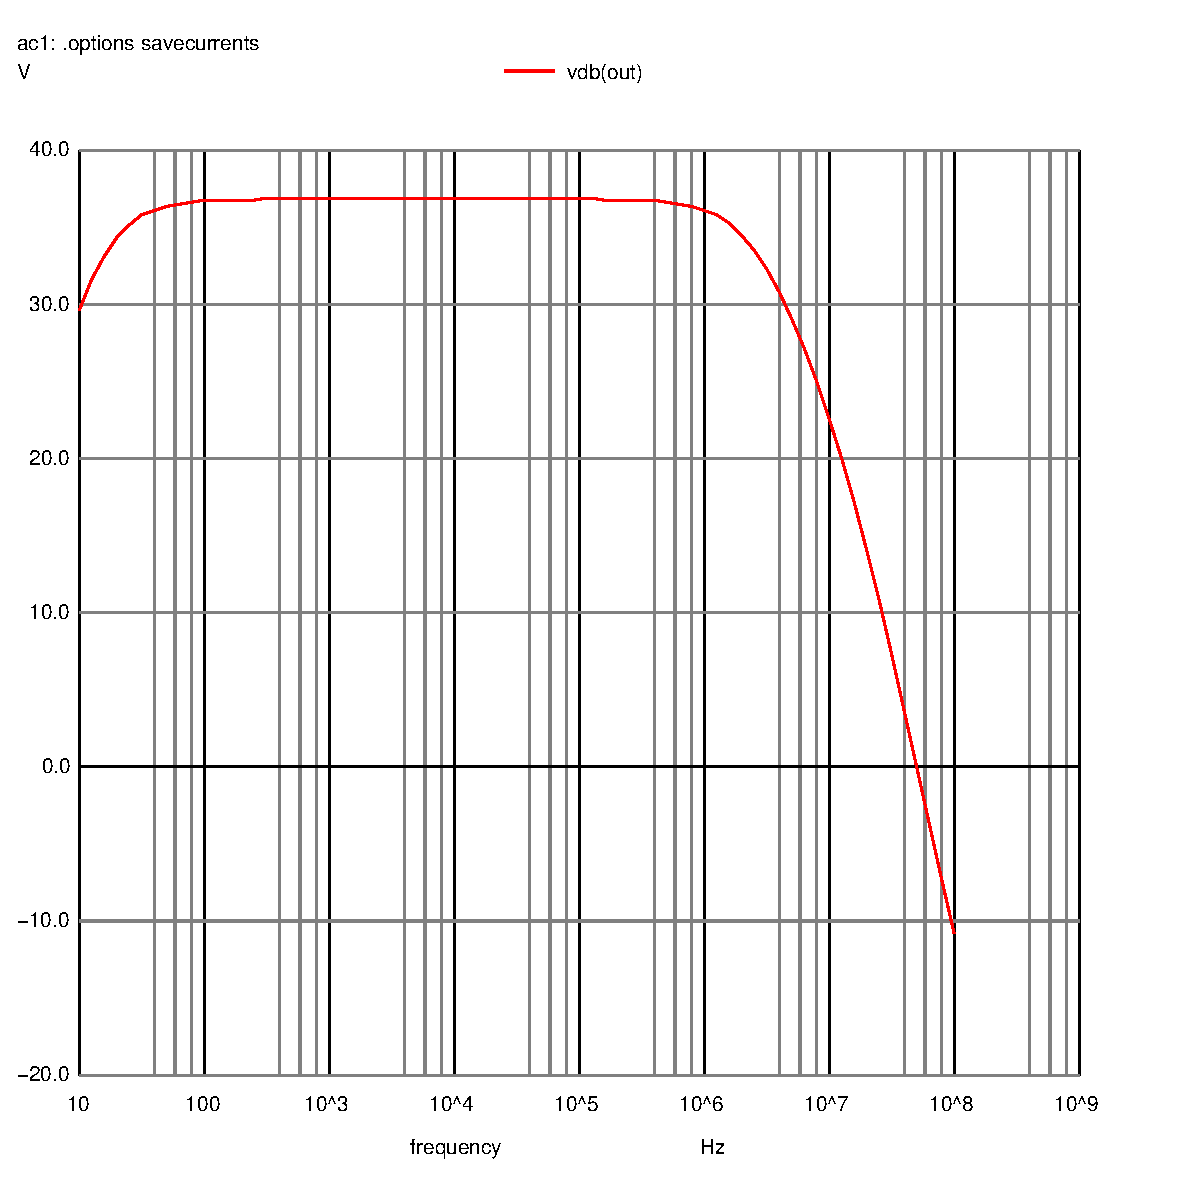
\includegraphics[width=0.4\linewidth]{out_gain.eps}
\caption{Output voltage gain}
\label{fig:gain_sim}
\end{figure}


\subsection{The input and output impedances}

\begin{figure}[ht!] \centering
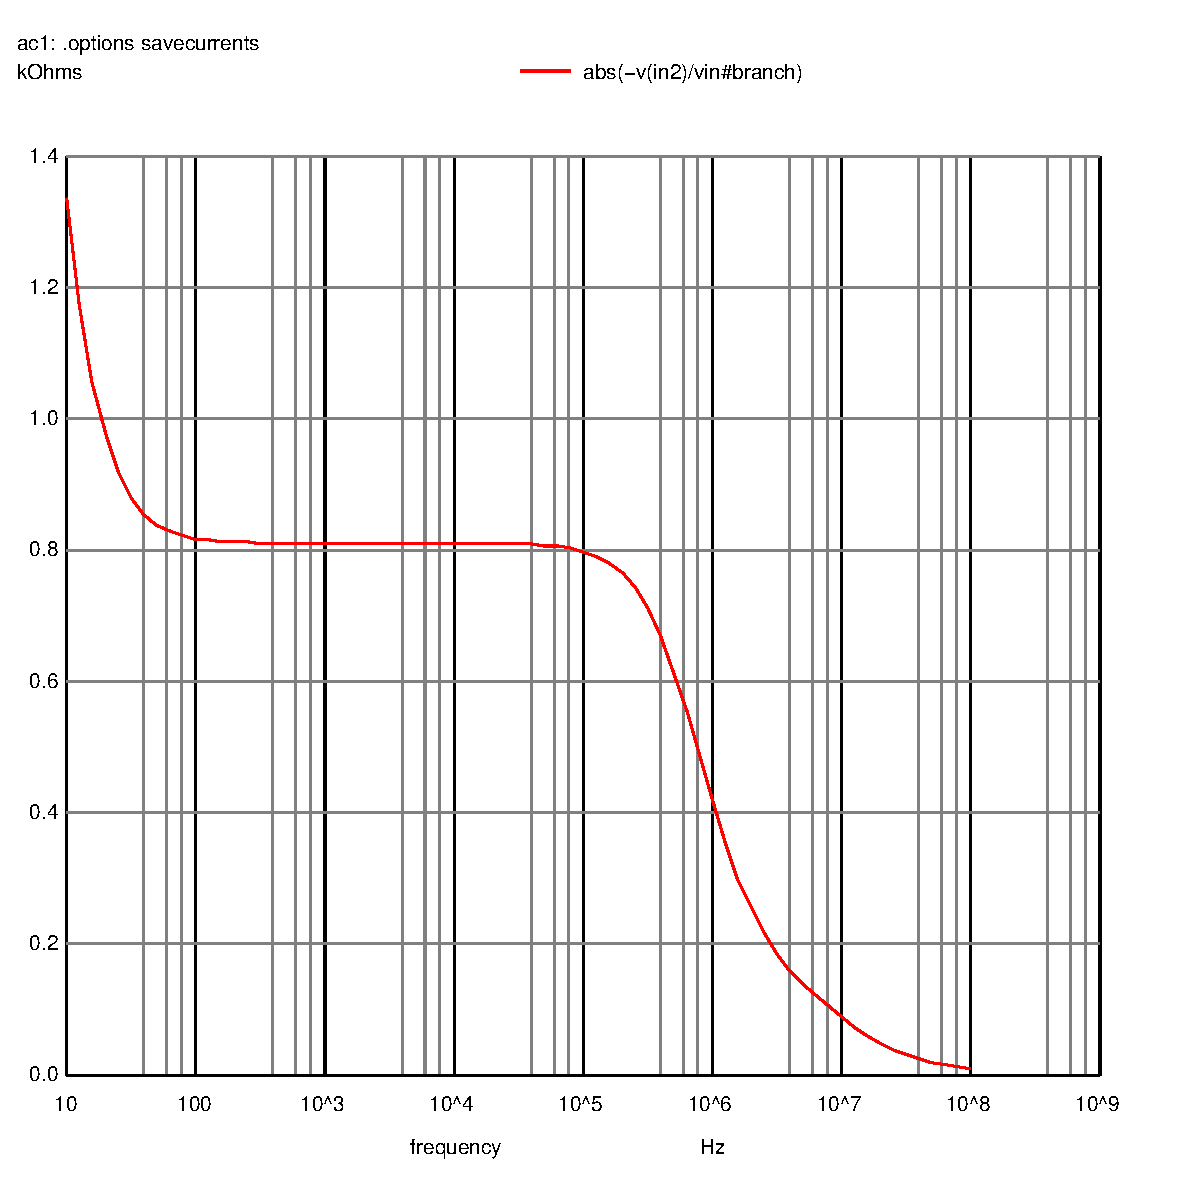
\includegraphics[width=0.4\linewidth]{impe_in.eps}
\caption{Input impedance }
\label{fig:In_imp}
\end{figure}

\begin{figure}[ht!] \centering
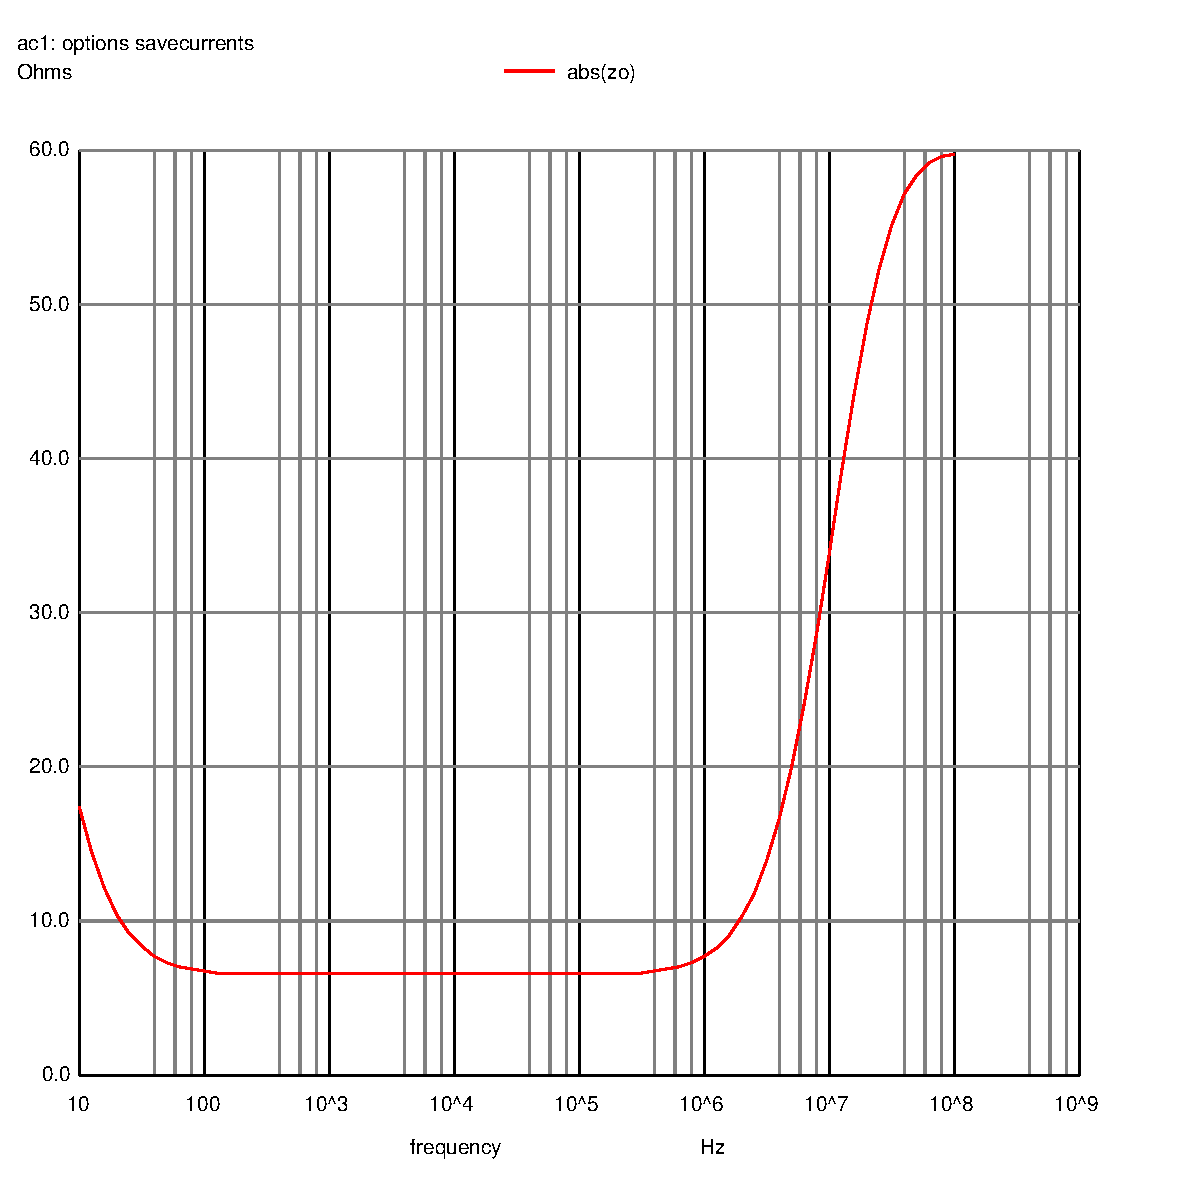
\includegraphics[width=0.4\linewidth]{impe_out.eps}
\caption{Output impedance }
\label{fig:out_imp}
\end{figure}




